\documentclass[10pt,a4paper]{article}
\pdfmapfile{+cm.map}

\usepackage[utf8]{inputenc}
\usepackage[provide=*,spanish]{babel}
\usepackage[margin=2cm,top=2.4cm,bottom=2cm]{geometry}
\usepackage{graphicx}
\usepackage{booktabs}
\usepackage{float}
\usepackage{enumitem}
\usepackage{fancyhdr}
\usepackage{caption}
\usepackage{multirow}
\usepackage[hidelinks]{hyperref}
\usepackage{url}

\captionsetup{font=small,labelfont=bf}
\setlist[itemize]{leftmargin=1.2em,itemsep=2pt,topsep=3pt,parsep=0pt}
\setlength{\parskip}{3pt}
\setlength{\parindent}{0pt}

\pagestyle{fancy}
\fancyhf{}
\fancyhead[L]{\footnotesize CC3084 -- Data Science --- Laboratorio 4: Análisis de datos geoespaciales}
\fancyhead[R]{\footnotesize UVG -- Semestre II, 2026}
\fancyfoot[C]{\thepage}
\renewcommand{\headrulewidth}{0.4pt}

\begin{document}

\begin{center}
{\LARGE\bfseries Monitoreo satelital de cianobacterias en los lagos\\[2pt]
de Atitlán y Amatitlán}\\[6pt]
{\normalsize Laboratorio 4 -- CC3084 Data Science -- Sección 20 -- Grupo \#7}\\[4pt]
{\small Marco Carbajal (23025) \quad Carlos Angel (23010) \quad Diego Monroy (23318)}\\[4pt]
{\small Código y datos: \url{https://github.com/monroyd1611/Laboratorio-4---Data-Science}}
\end{center}

\vspace{2pt}

\section{Qué se midió y cómo}

Las cianobacterias son microorganismos que, cuando el agua tiene exceso de nutrientes, temperatura alta y poco
movimiento, se multiplican hasta formar floraciones que pueden ser tóxicas. Medirlas con muestreos en campo es caro
y solo describe el punto donde se tomó la muestra, así que en este trabajo se usó observación satelital, que cubre
el lago completo y permite comparar fechas distintas con el mismo criterio.

\begin{itemize}
  \item \textbf{Datos:} 22 imágenes del satélite Sentinel-2 del programa Copernicus, 11 fechas por lago, entre enero
  de 2025 y julio de 2026. Son las fechas oficiales del laboratorio, todas con nubosidad baja.
  \item \textbf{Índice de cianobacteria (NDCI):} compara la luz que el agua refleja en el borde rojo y en el rojo,
  dos colores en los que la clorofila de las cianobacterias deja una huella clara. Se calculó con el script público
  de cianobacterias de Sentinel Hub, que además convierte el índice a clorofila-a en microgramos por litro, la
  unidad que se usa en calidad de agua.
  \item \textbf{Índices de apoyo:} el NDWI separa el agua de la tierra y sirve para medir solo dentro del lago, y el
  NDVI describe la vegetación del entorno.
  \item \textbf{Resolución:} cada dato corresponde a un cuadro de 10 por 10 metros de superficie, es decir 100
  metros cuadrados.
  \item \textbf{Umbral de floración:} se considera floración visible un NDCI mayor a 0.2, valor a partir del cual el
  agua ya presenta una carga alta de material fotosintético en suspensión.
\end{itemize}

\begin{figure}[H]
  \centering
  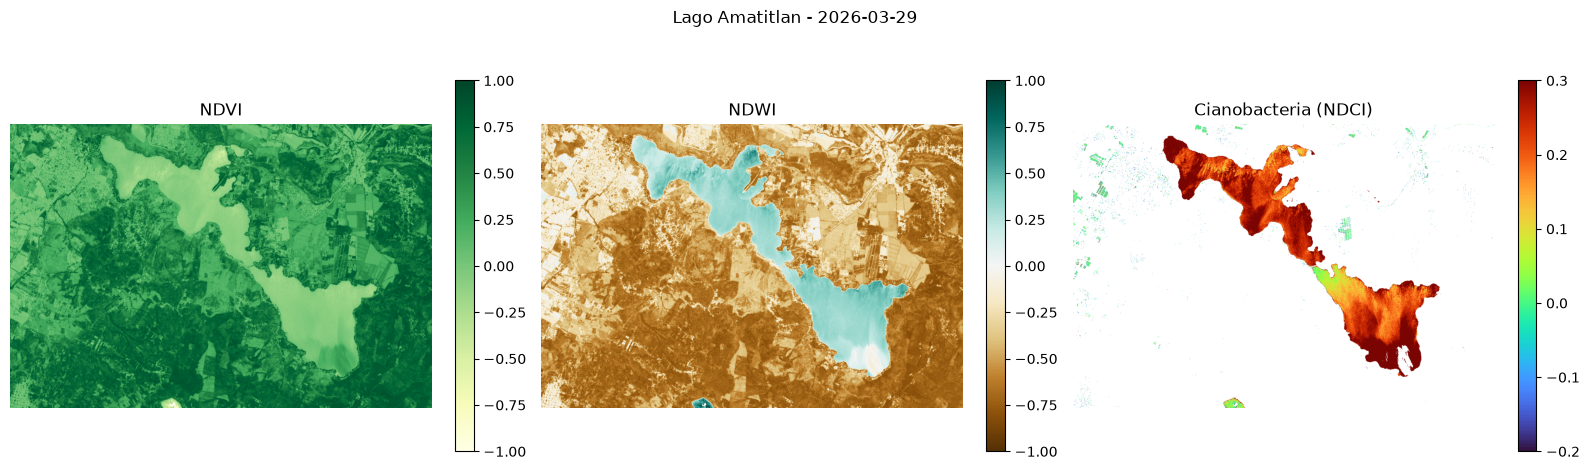
\includegraphics[width=0.95\linewidth]{figuras/indices_amatitlan.png}
  \caption{Los tres índices en el lago de Amatitlán el 29 de marzo de 2026. El NDVI (izquierda) muestra la
  vegetación del entorno, el NDWI (centro) delimita el espejo de agua y el mapa de cianobacteria (derecha) se
  calcula únicamente dentro de esa agua. El rojo indica concentraciones altas.}
\end{figure}

\section{Estado general de los dos lagos}

Los dos lagos están en situaciones opuestas, y la diferencia no es de matiz sino de un orden de magnitud.

\begin{table}[H]
  \centering
  \small
  \begin{tabular}{lcccccc}
    \toprule
    Lago & NDCI promedio & NDCI máximo & Clorofila-a media & Clorofila-a máxima & Fechas con & Superficie \\
     & & & (ug/L) & (ug/L) & floración & afectada \\
    \midrule
    Atitlán   & $-0.026$ & 0.014 & 3.5  & 4.3  & 0 de 11 & 5\%  \\
    Amatitlán & 0.217    & 0.397 & 12.5 & 54.2 & 5 de 11 & 55\% \\
    \bottomrule
  \end{tabular}
  \caption{Resumen de las 11 fechas de cada lago. La superficie afectada es el porcentaje promedio del espejo de
  agua que supera el umbral de floración.}
\end{table}

Amatitlán presenta valores propios de un lago hipereutrófico, es decir con exceso permanente de nutrientes: su
clorofila-a promedio de 12.5 microgramos por litro triplica a la de Atitlán y en la peor fecha llega a 54.2.
Atitlán se mantiene entre 3 y 4 microgramos por litro en todas las fechas, un nivel de agua limpia, y ninguna de
sus imágenes alcanza el umbral de floración.

\section{Cómo cambió en el tiempo}

\begin{figure}[H]
  \centering
  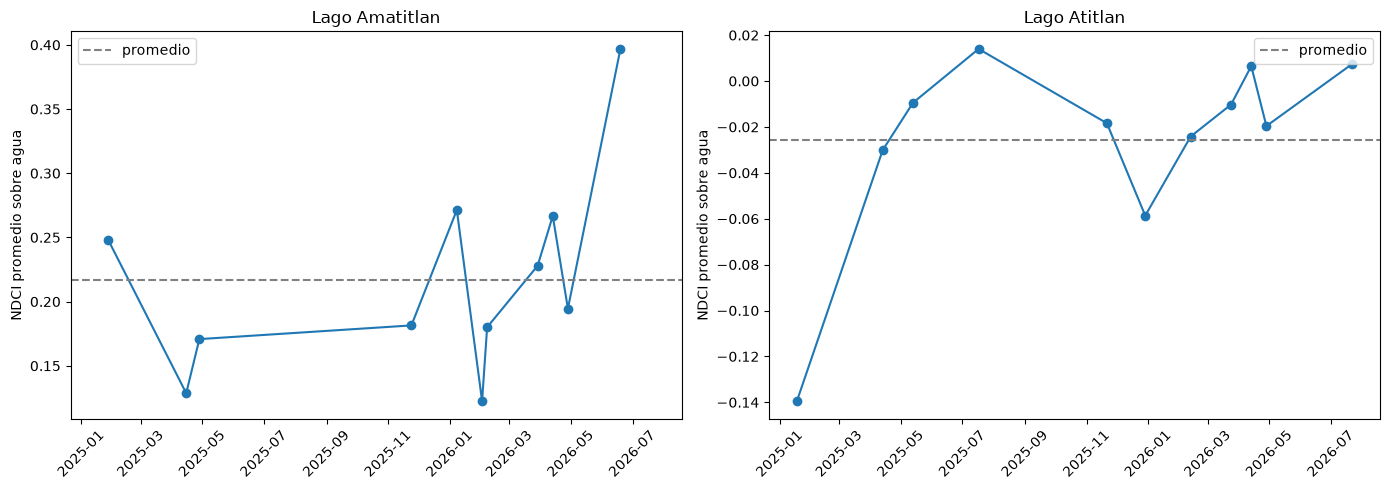
\includegraphics[width=0.95\linewidth]{figuras/serie_temporal.png}
  \caption{Evolución del índice de cianobacteria en cada lago. La línea punteada es el promedio del periodo. Las
  escalas verticales son distintas: el rango completo de Atitlán cabe dentro de las fluctuaciones de Amatitlán.}
\end{figure}

En Amatitlán la serie fluctúa mucho, pero siempre en niveles altos: baja hasta 0.12 en abril de 2025 y febrero de
2026, y sube a 0.27 en enero y abril de 2026. El pico del periodo es el 19 de junio de 2026, con un índice de 0.397
y 54.2 microgramos por litro de clorofila-a, la única fecha que supera el criterio de floración excepcional,
definido como el promedio del lago más una desviación estándar. Es también la única fecha del periodo que cae en
época lluviosa, cuando la escorrentía arrastra nutrientes y el agua está más caliente. Con una sola observación de
esa temporada no se puede afirmar un patrón estacional, pero la dirección coincide con lo esperado. Vale la pena
señalar que el promedio de las fechas de 2026, de 0.24, es mayor que el de 2025, de 0.18.

En Atitlán la serie se mantiene plana alrededor de cero durante los dos años, sin ningún pico. Sus valores más
altos, que aun así son bajos, caen en julio de 2025, abril de 2026 y julio de 2026.

\begin{table}[H]
  \centering
  \small
  \begin{minipage}[t]{0.48\linewidth}
    \centering
    \begin{tabular}{lccc}
      \toprule
      \multicolumn{4}{c}{\textbf{Lago de Atitlán}} \\
      \midrule
      Fecha & NDCI & Clorofila & Superficie \\
            &      & (ug/L)    & afectada \\
      \midrule
      2025-01-18 & $-0.139$ & 0.0 & 24.2\% \\
      2025-04-13 & $-0.030$ & 3.4 & 0.6\%  \\
      2025-05-13 & $-0.009$ & 4.0 & 0.5\%  \\
      2025-07-17 & 0.014    & 4.3 & 1.7\%  \\
      2025-11-21 & $-0.018$ & 4.1 & 12.9\% \\
      2025-12-29 & $-0.059$ & 3.1 & 4.4\%  \\
      2026-02-12 & $-0.024$ & 3.7 & 6.0\%  \\
      2026-03-24 & $-0.010$ & 3.9 & 0.7\%  \\
      2026-04-13 & 0.006    & 4.3 & 0.7\%  \\
      2026-04-28 & $-0.020$ & 3.7 & 0.5\%  \\
      2026-07-22 & 0.007    & 4.2 & 1.0\%  \\
      \bottomrule
    \end{tabular}
  \end{minipage}
  \hfill
  \begin{minipage}[t]{0.48\linewidth}
    \centering
    \begin{tabular}{lccc}
      \toprule
      \multicolumn{4}{c}{\textbf{Lago de Amatitlán}} \\
      \midrule
      Fecha & NDCI & Clorofila & Superficie \\
            &      & (ug/L)    & afectada \\
      \midrule
      2025-01-28 & 0.248 & 11.7 & 76.0\% \\
      2025-04-15 & 0.129 & 5.0  & 28.7\% \\
      2025-04-28 & 0.171 & 5.4  & 42.7\% \\
      2025-11-24 & 0.181 & 6.3  & 37.9\% \\
      2026-01-08 & 0.271 & 14.2 & 81.1\% \\
      2026-02-02 & 0.122 & 5.3  & 14.6\% \\
      2026-02-07 & 0.180 & 6.9  & 41.0\% \\
      2026-03-29 & 0.228 & 9.6  & 68.0\% \\
      2026-04-13 & 0.267 & 13.6 & 88.4\% \\
      2026-04-28 & 0.195 & 5.2  & 41.1\% \\
      2026-06-19 & 0.397 & 54.2 & 87.0\% \\
      \bottomrule
    \end{tabular}
  \end{minipage}
  \caption{Resultados fecha por fecha. La imagen de Atitlán del 18 de enero de 2025 no es comparable con el resto
  por las razones que se explican en la sección de limitaciones.}
\end{table}

\section{Dónde se concentra la floración dentro del lago}

El promedio de un lago esconde lo más útil para el manejo, que es saber dónde ocurre el problema. Al superponer las
11 fechas de Amatitlán aparece un patrón muy estable.

\begin{figure}[H]
  \centering
  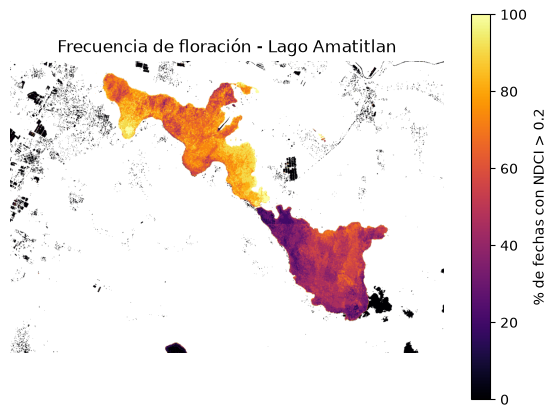
\includegraphics[width=0.56\linewidth]{figuras/frecuencia_amatitlan.png}
  \caption{Porcentaje de las 11 fechas en que cada punto del lago de Amatitlán superó el umbral de floración. La
  cuenca norte, donde desemboca el río Villalobos, aparece en amarillo y naranja; la cuenca sur, del lado de la
  salida hacia el río Michatoya, se mantiene más limpia.}
\end{figure}

Sobre los 14.3 kilómetros cuadrados de agua permanente del lago, la mitad norte promedia un índice de 0.264 y la
mitad sur 0.192. El diez por ciento de los puntos con mayor carga promedia 0.323 y se ubica en la cuenca
norponiente, justo donde entra el río Villalobos con el drenaje del área metropolitana. Esa mitad norte supera el
umbral en cerca del 71 por ciento de las fechas, contra el 44 por ciento de la mitad sur. No se trata de un episodio
aislado sino de una zona de acumulación permanente, y es el sitio donde tendría más sentido concentrar el muestreo
en campo y las alertas al público.

\begin{figure}[H]
  \centering
  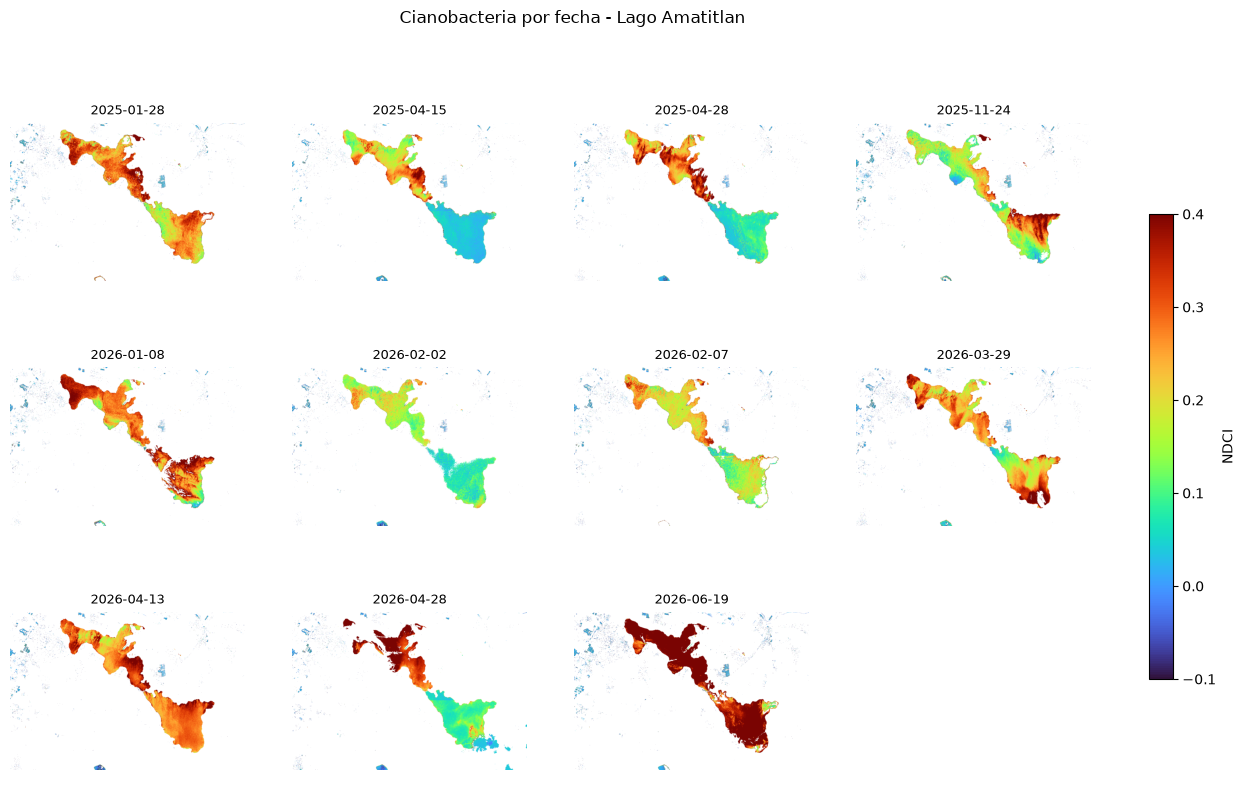
\includegraphics[width=0.92\linewidth]{figuras/rejilla_amatitlan.png}
  \caption{Las 11 fechas del lago de Amatitlán en la misma escala de color. Lo que cambia entre fechas es la
  intensidad, no la ubicación: la cuenca norte siempre aparece más cargada que la sur.}
\end{figure}

En Atitlán no existe ningún patrón equivalente. El promedio de las 11 fechas es plano en todo el espejo de agua y
los puntos más altos y más bajos se ubican prácticamente en el mismo lugar, lo que indica ruido de medición y no una
estructura real. Los únicos valores que superan el umbral forman una franja delgada pegada a la orilla, donde el
cuadro de 10 metros mezcla agua con vegetación ribereña y por eso el índice sube de forma artificial.

\section{Cuánta superficie cubren las floraciones}

\begin{figure}[H]
  \centering
  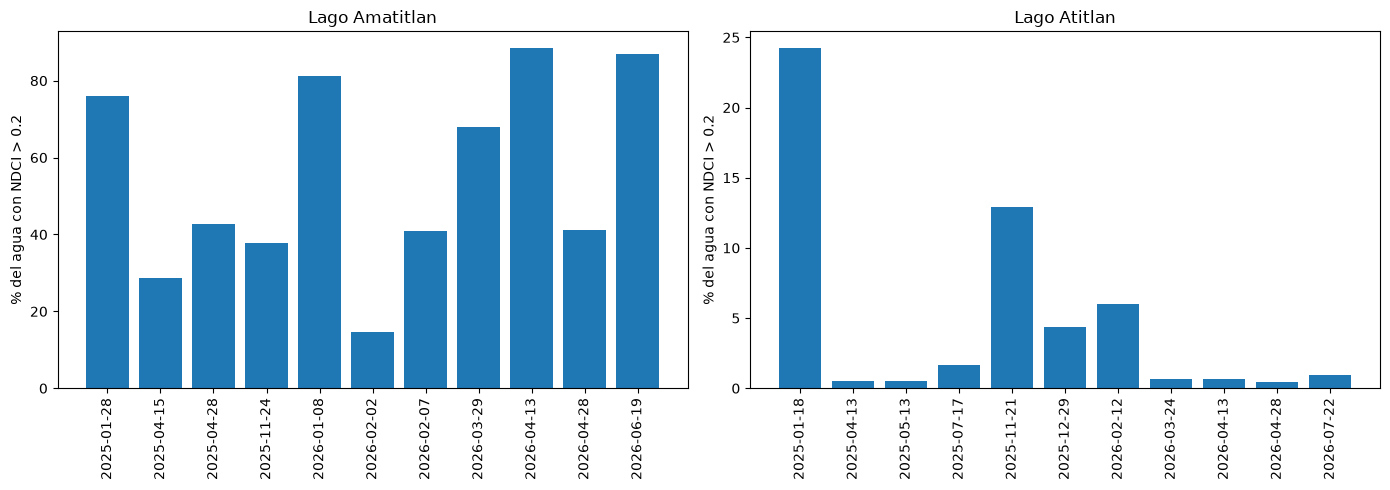
\includegraphics[width=0.95\linewidth]{figuras/extension_floracion.png}
  \caption{Porcentaje del espejo de agua con floración en cada fecha. En Amatitlán, seis de las once fechas superan
  el 40 por ciento del lago. Las escalas verticales son distintas.}
\end{figure}

En Amatitlán la extensión va del 15 por ciento en febrero de 2026 al 88 por ciento en abril de 2026, y en seis de
las once fechas más del 40 por ciento del lago está afectado. La floración de junio de 2026 no es una mancha local:
cubre prácticamente todo el espejo de agua, y el aumento respecto a febrero es positivo en toda la superficie.

En Atitlán los valores parecen altos en cuatro fechas, con 24.2 por ciento en enero de 2025 y 12.9 por ciento en
noviembre de 2025, pero esas cuatro fechas son exactamente las cuatro imágenes con menos píxeles útiles por bruma y
sombra. Son artefactos de la imagen y no floraciones reales, y conviene tenerlo presente porque es el tipo de dato
que puede llevar a una alerta equivocada.

\section{Comparación entre los dos lagos}

\begin{figure}[H]
  \centering
  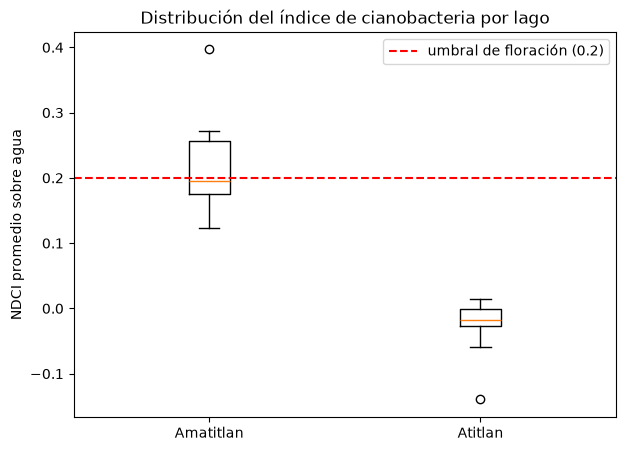
\includegraphics[width=0.45\linewidth]{figuras/boxplot_lagos.png}
  \caption{Distribución del índice en las 11 fechas de cada lago. Las dos distribuciones no se traslapan y solo
  Amatitlán cruza el umbral de floración.}
\end{figure}

\begin{itemize}
  \item \textbf{Intensidad:} Amatitlán promedia 0.217 y llega a 0.397, contra un promedio de $-0.026$ y un máximo de
  0.014 en Atitlán. En clorofila-a la diferencia es de 12.5 frente a 3.5 microgramos por litro en promedio.
  \item \textbf{Frecuencia:} 5 de las 11 fechas de Amatitlán superan el umbral y ninguna de Atitlán lo hace. En
  Amatitlán la floración no es un evento, es un estado permanente que solo cambia de intensidad.
  \item \textbf{Extensión:} 55 por ciento del lago afectado en promedio en Amatitlán, contra 5 por ciento en
  Atitlán, y ese 5 por ciento corresponde a la orilla y a las fechas con bruma.
\end{itemize}

\section{Qué explica la diferencia}

Las causas apuntan a la presión urbana y a la forma misma de cada lago.

\begin{itemize}
  \item \textbf{Carga de nutrientes:} Amatitlán recibe por el río Villalobos el drenaje de la cuenca metropolitana,
  con aguas residuales en su mayoría sin tratamiento, descargas industriales y escorrentía de suelo urbanizado y
  agrícola. Ese aporte entra por la orilla norte, que es precisamente la de mayor carga en los mapas.
  \item \textbf{Volumen y profundidad:} Amatitlán tiene unos 15 kilómetros cuadrados y poca profundidad, mientras
  que Atitlán supera los 100 kilómetros cuadrados y varios cientos de metros de profundidad, de modo que el mismo
  aporte de nutrientes se diluye en un volumen mucho mayor.
  \item \textbf{Temperatura y altitud:} Amatitlán está a menor altitud y su agua es más cálida, condición que
  favorece el crecimiento de las cianobacterias durante todo el año.
  \item \textbf{Uso del suelo:} la cuenca de Atitlán es menos poblada y conserva más bosque y cultivo de café, con
  una presión sobre el agua mucho menor que la del corredor urbano que drena hacia Amatitlán.
\end{itemize}

\section{Modelos de clasificación}

La unidad de modelado es un píxel válido de agua de 10 por 10 metros. La variable respuesta toma el valor 1 cuando
la clorofila-a estimada es al menos 12 microgramos por litro, entrada al Nivel de Alerta 1, y 0 en caso contrario.
El conjunto contiene 450,499 observaciones de 21 fechas; la imagen de Atitlán del 18 de enero de 2025 se excluyó
porque solo conservó 2.98\% de cobertura válida. La clase positiva representa 6.15\%, por lo que la exactitud por sí
sola no es un criterio suficiente.

Se utilizaron B03, B04, B08, NDVI, NDWI, los cocientes verde/rojo y NIR/verde, brillo, textura local del NDWI y
distancia a la orilla. Se excluyeron clorofila-a, NDCI y B05: las dos primeras definen directamente la respuesta y
B05, junto con B04, permite reconstruir NDCI. También se excluyeron lago, fecha, latitud y longitud para evitar que
los modelos memorizaran la ubicación en vez de aprender la firma espectral.

\subsection{Entrenamiento y comparación justa}

Se hizo una única división estratificada y reproducible: 70\% para entrenamiento y 30\% para prueba, con semilla 42.
Los tres algoritmos ---Regresión Logística, Random Forest y Gradient Boosting por histogramas--- recibieron
exactamente los mismos índices de prueba. Primero se entrenaron con su configuración inicial y umbral 0.5. Después,
el ajuste de hiperparámetros se realizó exclusivamente dentro del 70\% de entrenamiento mediante validación
estratificada de tres particiones. El conjunto de prueba no intervino ni en la selección de parámetros ni en la
elección del umbral.

Debido al tamaño del conjunto, la búsqueda se realizó sobre una submuestra estratificada de 120,000 observaciones
del entrenamiento y la configuración elegida se volvió a ajustar con todo el 70\%. Los valores evaluados fueron:

\begin{itemize}
  \item \textbf{Regresión Logística:} $C\in\{0.01,0.1,1,10\}$ y pesos de clase nulos o balanceados. Las variables
  se estandarizaron dentro de un \textit{pipeline} para que la escala se aprendiera sin observar la prueba.
  \item \textbf{Random Forest:} 250 árboles; profundidad máxima de 12, 24 o sin límite; mínimo de 1, 5 o 20
  observaciones por hoja; número de variables por división igual a la raíz del total o 70\%; y pesos nulos o
  balanceados por submuestra. Se evaluaron diez combinaciones aleatorias con semilla fija.
  \item \textbf{Gradient Boosting:} tasa de aprendizaje de 0.03, 0.07 o 0.12; 100 o 200 iteraciones; 15, 31 o 63
  hojas; mínimo de 20 o 100 observaciones por hoja; regularización L2 de 0 o 1; y pesos de clase nulos o balanceados.
  Se evaluaron diez combinaciones aleatorias con semilla fija.
\end{itemize}

El criterio de selección fue F2, que da al \textit{recall} el doble de importancia que a la precisión. Luego se
reservó 15\% del entrenamiento como validación interna para elegir, entre 0.05 y 0.95, el umbral que maximizó F2;
por último cada modelo se reentrenó con todo el entrenamiento antes de evaluarlo una sola vez en la prueba.

\subsection{Criterio ambiental de evaluación}

Un falso positivo marca como alta presencia una zona que no la tiene. Esto puede producir una alerta innecesaria,
muestreos adicionales, gasto operativo y pérdida de confianza si se repite. Un falso negativo omite una zona que sí
tiene alta presencia, lo cual puede retrasar el muestreo confirmatorio y mantener la exposición recreativa o el uso
del agua ante una floración potencialmente tóxica. Para un sistema de alerta temprana se considera más importante
reducir falsos negativos. Por ello la comparación principal usa F2 y \textit{recall}; ROC-AUC se reporta como medida
general de discriminación, pero no representa por sí sola el costo desigual de los dos errores.

\subsection{Resultados iniciales}

Con umbral 0.5 y antes del ajuste, Random Forest presentó el mayor F2 y F1. La exactitud de los tres modelos fue
alta, pero debe interpretarse junto con el \textit{recall}: por el desbalance, un modelo puede acertar la mayoría de
los negativos y aun así omitir muchas zonas afectadas.

\begin{table}[H]
  \centering
  \small
  \begin{tabular}{lrrrrrr}
    \toprule
    Modelo & Accuracy & Precision & Recall & F1 & F2 & ROC-AUC \\
    \midrule
    Regresión Logística & 0.954 & 0.741 & 0.396 & 0.516 & 0.436 & 0.884 \\
    Random Forest       & 0.971 & 0.843 & 0.657 & 0.738 & 0.687 & 0.979 \\
    Gradient Boosting   & 0.970 & 0.843 & 0.632 & 0.722 & 0.665 & 0.981 \\
    \bottomrule
  \end{tabular}
  \caption{Desempeño inicial sobre las mismas 135,150 observaciones de prueba, usando umbral 0.5.}
\end{table}

\subsection{Configuraciones seleccionadas}

La búsqueda eligió $C=10$ y pesos balanceados para Regresión Logística. Para Random Forest seleccionó profundidad
24, mínimo de 20 observaciones por hoja, 70\% de variables por división y pesos balanceados por submuestra. Para
Gradient Boosting eligió tasa 0.03, 200 iteraciones, 63 hojas, mínimo de 20 observaciones por hoja, regularización
L2 igual a 0 y pesos balanceados. Los F2 medios de validación cruzada fueron 0.582, 0.773 y 0.764,
respectivamente. Los umbrales seleccionados en la validación interna fueron 0.600, 0.595 y 0.725.

\subsection{Resultados finales}

\begin{table}[H]
  \centering
  \small
  \begin{tabular}{lrrrrrr}
    \toprule
    Modelo & Accuracy & Precision & Recall & F1 & F2 & ROC-AUC \\
    \midrule
    Regresión Logística & 0.912 & 0.381 & 0.701 & 0.493 & 0.600 & 0.913 \\
    Random Forest       & 0.954 & 0.588 & 0.870 & 0.702 & 0.794 & 0.982 \\
    Gradient Boosting   & 0.950 & 0.558 & 0.880 & 0.683 & 0.789 & 0.982 \\
    \bottomrule
  \end{tabular}
  \caption{Desempeño final sobre el conjunto común de prueba después del ajuste.}
\end{table}

\begin{figure}[H]
  \centering
  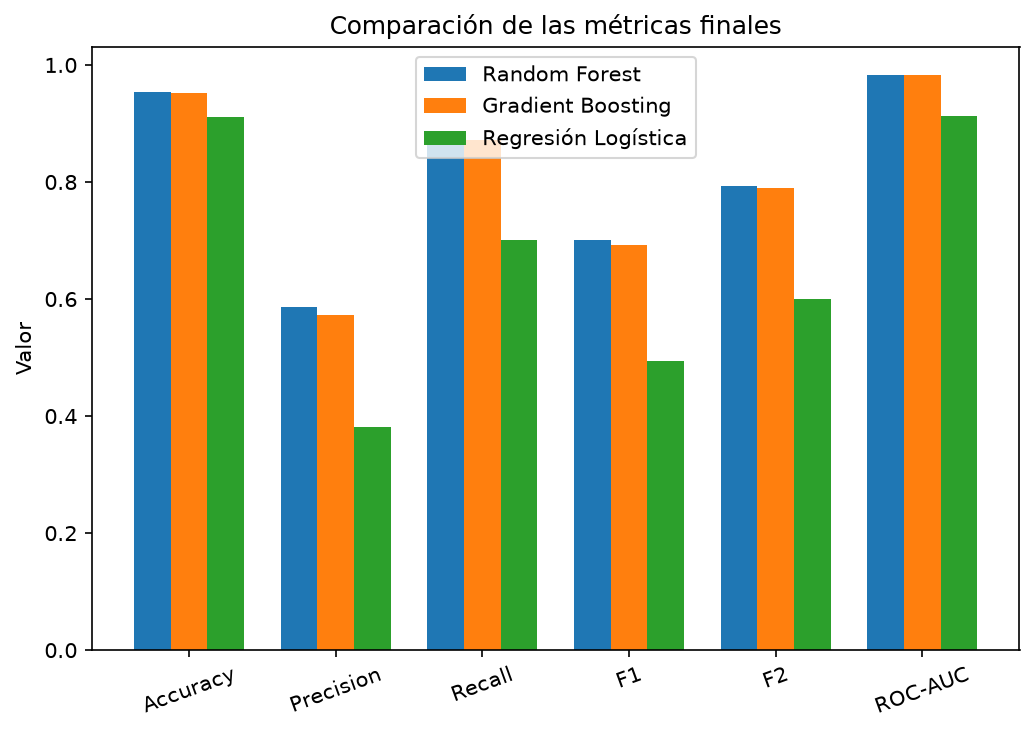
\includegraphics[width=0.98\linewidth]{figuras/comparacion_modelos.png}
  \caption{Comparación de las métricas finales. Random Forest y Gradient Boosting superan claramente a la
  Regresión Logística en \textit{recall}, F1, F2 y ROC-AUC.}
\end{figure}

\begin{table}[H]
  \centering
  \small
  \begin{tabular}{lrrrrr}
    \toprule
    Modelo & Umbral & TN & FP & FN & TP \\
    \midrule
    Regresión Logística & 0.600 & 117,368 & 9,467 & 2,490 & 5,825 \\
    Random Forest       & 0.595 & 121,763 & 5,072 & 1,079 & 7,236 \\
    Gradient Boosting   & 0.725 & 121,046 & 5,789 &   994 & 7,321 \\
    \bottomrule
  \end{tabular}
  \caption{Matrices de confusión finales expresadas como conteos: verdaderos negativos (TN), falsos positivos
  (FP), falsos negativos (FN) y verdaderos positivos (TP).}
\end{table}

\begin{figure}[H]
  \centering
  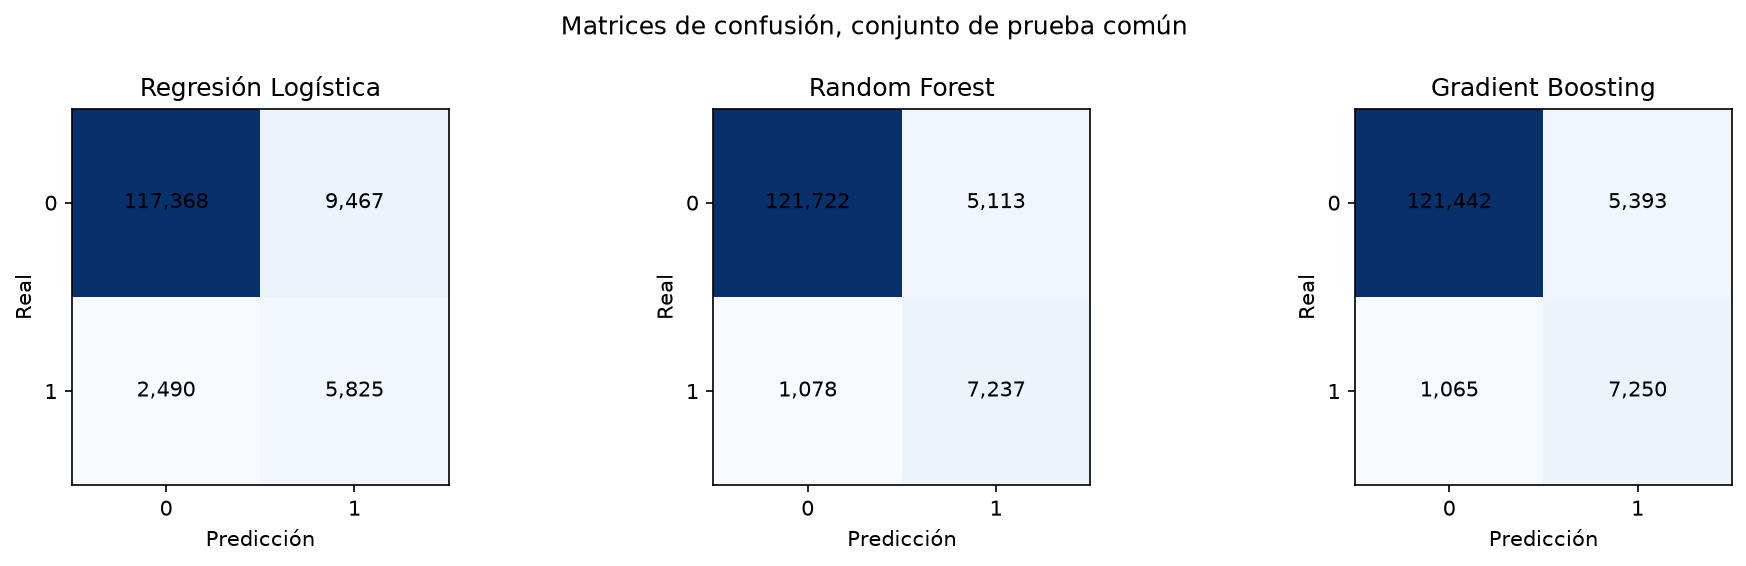
\includegraphics[width=0.98\linewidth]{figuras/matrices_confusion_modelos.png}
  \caption{Matrices de confusión de los modelos ajustados sobre las mismas 135,150 observaciones de prueba.}
\end{figure}

Random Forest es el modelo final recomendado: alcanza el mayor F2 (0.794), el mayor ROC-AUC (0.9824) y mantiene
un \textit{recall} de 0.870 con menos falsos positivos que Gradient Boosting. Gradient Boosting detecta 85 positivos
adicionales y reduce los falsos negativos de 1,079 a 994, pero genera 717 falsos positivos más; su F2 queda
ligeramente por debajo, en 0.789. Si la política operativa exigiera minimizar los falsos negativos casi sin importar
el costo de inspección, Gradient Boosting sería defendible por su \textit{recall} de 0.880. Bajo el balance ambiental
adoptado mediante F2, Random Forest ofrece la mejor relación entre detección y falsas alarmas.

\section{Validación espacial y temporal}

La validación aleatoria del inciso anterior asume que las observaciones de prueba son independientes de las de
entrenamiento, algo que no se cumple en un campo espacial continuo: un píxel de 10 metros comparte casi toda su
información con sus vecinos inmediatos. Para medir el efecto de esa autocorrelación se reproyectaron las
coordenadas a WGS 84 / UTM zona 15N (EPSG:32615), sistema métrico que corresponde a la longitud de ambos lagos, y
se construyó una cuadrícula de bloques sobre la cual aplicar una validación cruzada agrupada.

\subsection{Tamaño de bloque}

Se probaron cuadrículas de 500, 1000, 1500 y 2000 metros (tabla \ref{tab:tamano-bloque}). Con 500 m el 5.6\% de los
bloques de Amatitlán queda con menos de 5 observaciones; con 2000 m un solo bloque llega a concentrar hasta 16,028
observaciones mientras otros tienen menos de 10, lo que produce folds muy desiguales. El tamaño de 1000 metros da el
mejor balance: 39 bloques en Amatitlán y 164 en Atitlán, suficientes para una validación cruzada agrupada de 5
particiones con varios bloques por fold en los dos lagos, y solo 2.6\% y 0.6\% de bloques casi vacíos.

\begin{table}[H]
  \centering
  \small
  \begin{tabular}{rlrrrr}
    \toprule
    Tamaño (m) & Lago & Bloques & Obs. mediana & Obs. máx. & Bloques con \\
     & & & & & $<$5 obs. (\%) \\
    \midrule
    500  & Amatitlán & 107 & 524   & 1,155  & 5.6 \\
    500  & Atitlán   & 571 & 938   & 1,081  & 1.1 \\
    1000 & Amatitlán & 39  & 1,085 & 4,438  & 2.6 \\
    1000 & Atitlán   & 164 & 3,280 & 4,077  & 0.6 \\
    1500 & Amatitlán & 23  & 2,374 & 7,953  & 4.3 \\
    1500 & Atitlán   & 83  & 5,393 & 9,037  & 0.0 \\
    2000 & Amatitlán & 19  & 1,129 & 14,154 & 0.0 \\
    2000 & Atitlán   & 51  & 4,973 & 16,028 & 2.0 \\
    \bottomrule
  \end{tabular}
  \caption{Bloques y observaciones por bloque según el tamaño de cuadrícula probado.}
  \label{tab:tamano-bloque}
\end{table}

\begin{figure}[H]
  \centering
  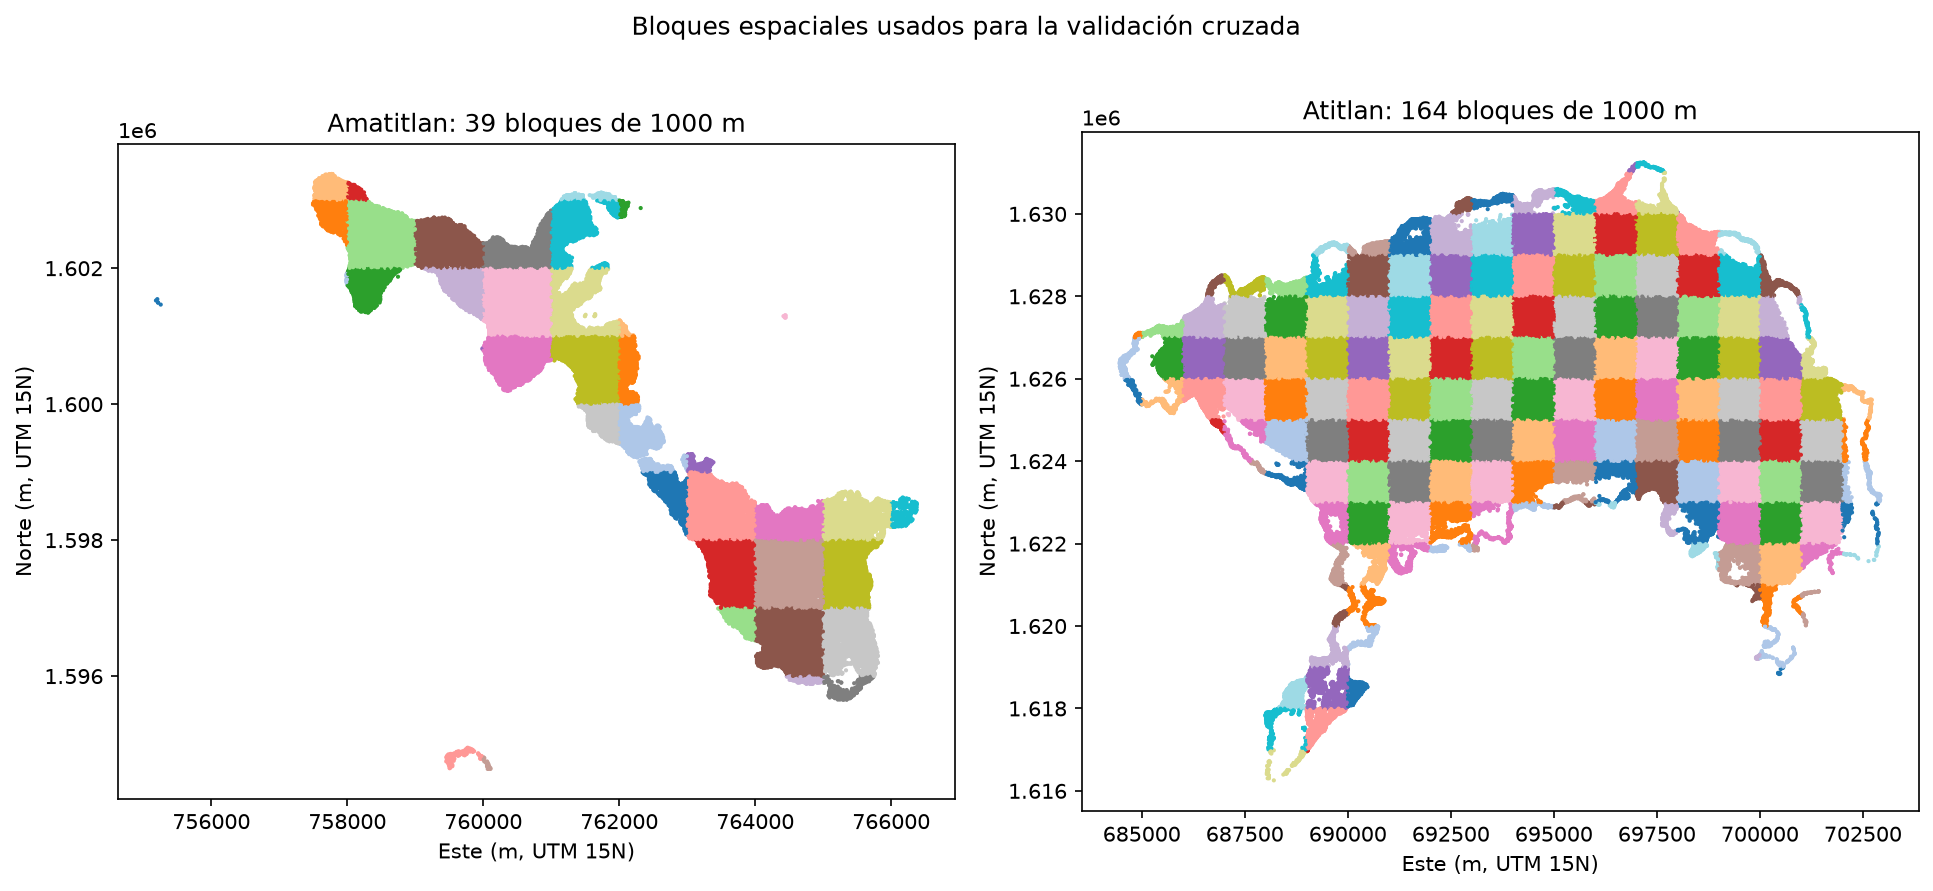
\includegraphics[width=0.95\linewidth]{figuras/bloques_espaciales.png}
  \caption{Bloques de 1000 m usados para la validación cruzada agrupada, un color distinto por bloque.}
\end{figure}

\subsection{Esquemas de validación comparados}

Se compararon tres esquemas sobre los mismos tres modelos ajustados en el inciso anterior, reutilizando sus
hiperparámetros y umbrales: la partición aleatoria 70/30 ya usada, una validación cruzada agrupada de 5 particiones
por bloque espacial (\texttt{GroupKFold} sobre el identificador de bloque, con las métricas promediadas entre las 5
particiones) y una partición temporal, entrenando con todas las fechas salvo la más reciente de cada lago y
evaluando sobre esa fecha más reciente (2026-06-19 en Amatitlán, 2026-07-22 en Atitlán).

\begin{table}[H]
  \centering
  \small
  \begin{tabular}{lrrrrrr}
    \toprule
    & \multicolumn{2}{c}{Aleatoria} & \multicolumn{2}{c}{Espacial (media 5 folds)} & \multicolumn{2}{c}{Temporal} \\
    \cmidrule(lr){2-3}\cmidrule(lr){4-5}\cmidrule(lr){6-7}
    Modelo & F2 & ROC-AUC & F2 & ROC-AUC & F2 & ROC-AUC \\
    \midrule
    Regresión Logística & 0.600 & 0.913 & 0.597 & 0.909 & 0.871 & 0.980 \\
    Random Forest       & 0.793 & 0.982 & 0.743 & 0.973 & 0.588 & 0.949 \\
    Gradient Boosting   & 0.790 & 0.982 & 0.753 & 0.974 & 0.586 & 0.957 \\
    \bottomrule
  \end{tabular}
  \caption{F2 y ROC-AUC bajo los tres esquemas de validación. La versión espacial es el promedio de 5 particiones;
  la desviación estándar entre ellas va de 0.030 a 0.057 en F2 según el modelo.}
\end{table}

Bajo validación espacial, el desempeño de los dos modelos de árboles baja y el de la Regresión Logística casi no se
mueve: Random Forest pasa de F2 0.793 a 0.743 (caída de 0.050) y Gradient Boosting de 0.790 a 0.753 (caída de
0.037), mientras la Regresión Logística pasa de 0.600 a 0.597. La causa es la autocorrelación espacial: bajo
partición aleatoria, un píxel de prueba casi siempre tiene vecinos de 10 metros en el entrenamiento con
reflectancia casi idéntica, y los modelos de árboles, más flexibles, aprovechan esa fuga para ajustarse a
combinaciones locales de las variables. La Regresión Logística, al ajustar una sola frontera lineal global, tiene
mucho menos margen para memorizar el vecindario, así que su estimación aleatoria ya era realista.

Bajo validación temporal el patrón se invierte: la Regresión Logística mejora mucho, hasta F2 0.871 con
\textit{recall} de 0.955, mientras Random Forest y Gradient Boosting caen a 0.588 y 0.586. La fecha de prueba de
Amatitlán, 2026-06-19, es el pico de floración de todo el periodo analizado en la Parte I (NDCI de 0.397 contra un
promedio del lago de 0.217), con reflectancias que superan todo lo visto en entrenamiento. Los modelos de árboles
particionan el espacio de variables con umbrales fijos aprendidos del rango de entrenamiento y no pueden extrapolar
más allá de ese rango, así que su \textit{recall} se desploma; la Regresión Logística, al ser lineal, sigue
extrapolando en la misma dirección más allá de lo observado, lo que en este caso coincide con la realidad de un
evento aún más extremo. Al depender de una sola fecha por lago, este resultado pesa más como prueba de estrés ante
un evento fuera de rango que como estimación estable del desempeño típico.

De los tres esquemas, la validación espacial da la estimación más realista de la capacidad del modelo para predecir
zonas nuevas dentro del periodo ya observado: aísla específicamente la fuga por autocorrelación espacial y promedia
5 particiones independientes, sin mezclar ese efecto con el problema distinto de la extrapolación a un régimen no
visto que sí afecta a la partición temporal.

\section{Generalización entre lagos}

Los dos lagos tienen prevalencias de la clase positiva y composiciones espectrales muy distintas. Esta sección mide
si un modelo entrenado únicamente con un lago clasifica correctamente al otro, reutilizando los mismos
hiperparámetros y umbrales ya elegidos, y lo compara contra el caso en que entrenamiento y prueba provienen del
mismo lago.

\begin{table}[H]
  \centering
  \small
  \begin{tabular}{llrrrrrr}
    \toprule
    Experimento & Modelo & Accuracy & Precision & Recall & F1 & F2 & ROC-AUC \\
    \midrule
    \multirow{3}{*}{Atitlán $\to$ Atitlán}
      & Regresión Logística & 0.943 & 0.154 & 0.933 & 0.264 & 0.463 & 0.982 \\
      & Random Forest       & 0.975 & 0.275 & 0.780 & 0.406 & 0.570 & 0.983 \\
      & Gradient Boosting   & 0.963 & 0.212 & 0.864 & 0.340 & 0.535 & 0.983 \\
    \multirow{3}{*}{Amatitlán $\to$ Amatitlán}
      & Regresión Logística & 0.838 & 0.825 & 0.756 & 0.789 & 0.769 & 0.920 \\
      & Random Forest       & 0.885 & 0.874 & 0.832 & 0.852 & 0.840 & 0.959 \\
      & Gradient Boosting   & 0.877 & 0.935 & 0.744 & 0.828 & 0.775 & 0.960 \\
    \bottomrule
  \end{tabular}
  \caption{Referencia: entrenamiento y prueba dentro del mismo lago (70\%/30\% estratificado).}
\end{table}

\begin{table}[H]
  \centering
  \small
  \begin{tabular}{llrrrrrr}
    \toprule
    Experimento & Modelo & Accuracy & Precision & Recall & F1 & F2 & ROC-AUC \\
    \midrule
    \multirow{3}{*}{Atitlán $\to$ Amatitlán (A)}
      & Regresión Logística & 0.610 & 0.597 & 0.074 & 0.132 & 0.090 & 0.695 \\
      & Random Forest       & 0.609 & 0.606 & 0.062 & 0.113 & 0.076 & 0.612 \\
      & Gradient Boosting   & 0.605 & 0.545 & 0.063 & 0.113 & 0.077 & 0.598 \\
    \multirow{3}{*}{Amatitlán $\to$ Atitlán (B)}
      & Regresión Logística & 0.358 & 0.016 & 0.920 & 0.031 & 0.073 & 0.802 \\
      & Random Forest       & 0.664 & 0.010 & 0.295 & 0.019 & 0.043 & 0.529 \\
      & Gradient Boosting   & 0.722 & 0.009 & 0.234 & 0.018 & 0.041 & 0.558 \\
    \bottomrule
  \end{tabular}
  \caption{Generalización cruzada: entrenamiento en un lago, prueba en el otro.}
\end{table}

Ningún modelo generaliza de un lago al otro. El F2 cae entre 8 y 13 veces frente al desempeño dentro del mismo
lago: de hasta 0.570 (Atitlán) y 0.840 (Amatitlán) dentro del mismo lago, a un máximo de 0.090 en el experimento A y
0.073 en el experimento B, ambos con la Regresión Logística. El tipo de error cambia según la dirección: en el
experimento A el problema es de \textit{recall} (0.06 a 0.07, contra 0.75-0.83 dentro del mismo lago), porque un
modelo entrenado donde solo 1.10\% de los píxeles son positivos casi no detecta la floración de Amatitlán; en el
experimento B el problema es de precisión (0.009 a 0.016, contra 0.15-0.27 dentro del mismo lago), porque un modelo
entrenado donde 39.94\% de los píxeles son positivos marca como floración una fracción enorme de los píxeles de
Atitlán que no lo son.

\subsection{Qué explica la diferencia}

\begin{figure}[H]
  \centering
  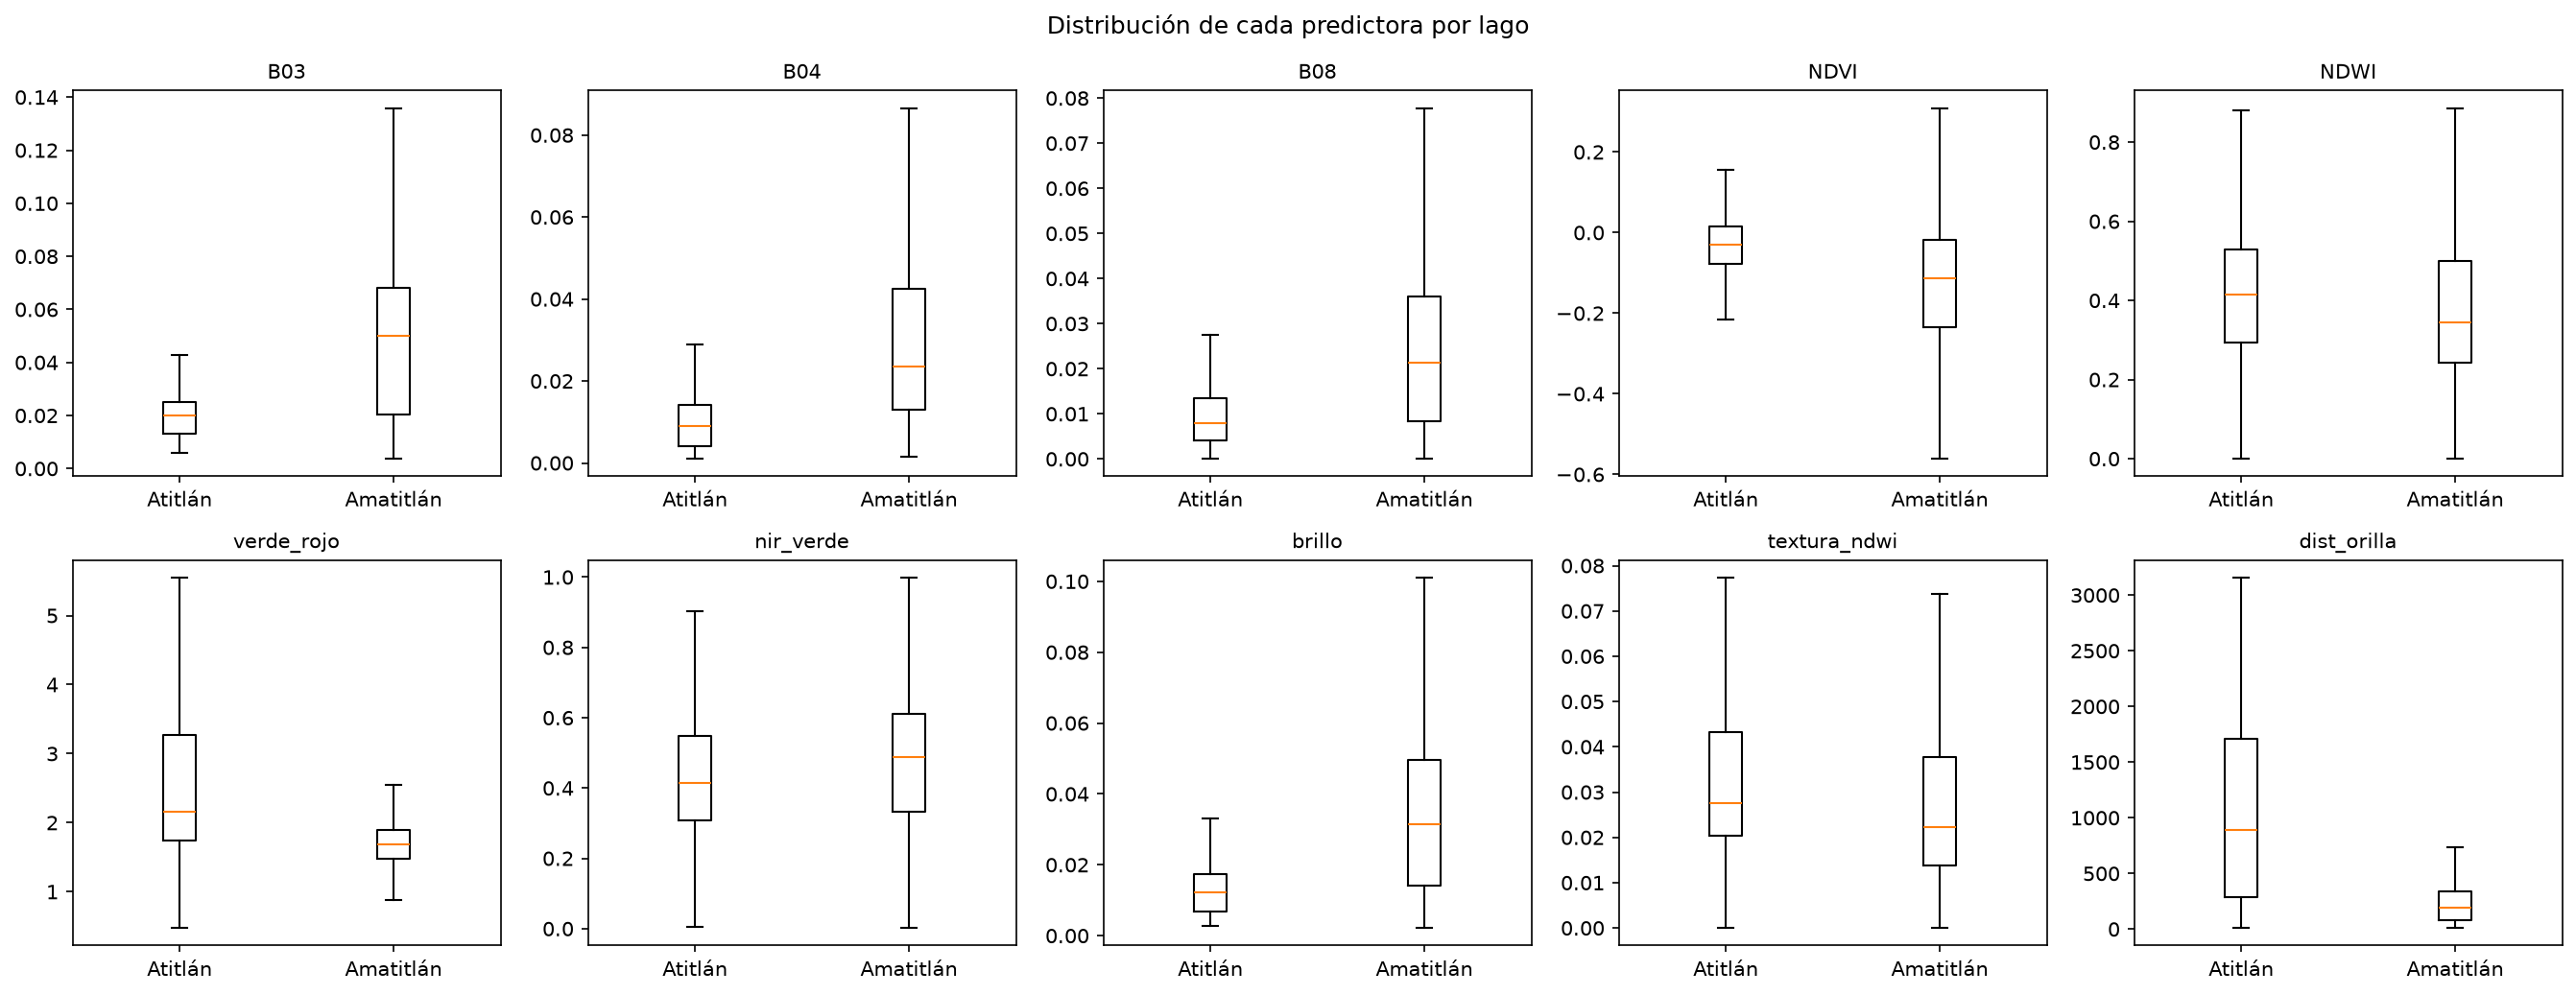
\includegraphics[width=0.95\linewidth]{figuras/comparacion_predictores_lagos.png}
  \caption{Distribución de cada predictora por lago, sin valores atípicos.}
\end{figure}

\begin{itemize}
  \item \textbf{Prevalencia:} 39.94\% de los píxeles de Amatitlán son de alta presencia contra 1.10\% en Atitlán,
  casi 36 veces más. Un modelo entrenado en un lago aprende un umbral de decisión calibrado para esa proporción, que
  queda mal calibrado en el otro.
  \item \textbf{Nivel de reflectancia:} B03, B04, B08 y brillo son entre 2.3 y 2.7 veces más altos en promedio en
  Amatitlán que en Atitlán (B03 pasa de 0.0205 a 0.0477); un valor moderado en un lago puede ser extremo en la
  escala del otro.
  \item \textbf{Distancia a la orilla:} promedia 1058 m en Atitlán contra 240 m en Amatitlán, casi 4.4 veces más,
  simple reflejo de que Atitlán es un lago mucho más extenso; el umbral de "cerca de la orilla" aprendido en un lago
  no es transferible al otro.
  \item \textbf{Tamaño, profundidad y eutrofización:} como se estableció en la Parte I, Amatitlán es pequeño y
  somero (unos 15 km²), recibe la descarga sin tratar del río Villalobos y se mantiene hipereutrófico (clorofila-a
  promedio de 12.5 ug/L); Atitlán es profundo, de origen volcánico, supera los cien kilómetros cuadrados y diluye
  cualquier aporte de nutrientes en un volumen mucho mayor, por lo que se mantiene oligotrófico (clorofila-a
  promedio de 3.5 ug/L).
\end{itemize}

En conjunto, la floración de cianobacterias en estos dos lagos no comparte una firma espectral única y portable:
depende del régimen de nutrientes propio de cada cuerpo de agua. Un sistema operativo de alerta temprana necesitaría
un modelo o al menos un umbral calibrado por lago, no un modelo entrenado en uno y aplicado directamente al otro.

\section{Interpretación y explicabilidad del modelo}

Se interpreta el Random Forest, que es el modelo con mejor F2. La importancia se mide por permutación sobre el
conjunto de prueba, barajando una variable a la vez y midiendo cuánto se degrada el F2, y se contrasta con los
valores SHAP, que reparten cada predicción individual entre las variables que la empujaron hacia arriba o hacia
abajo.

\begin{table}[H]
  \centering
  \small
  \begin{tabular}{lrrr}
    \toprule
    Variable & Caída de F2 & SHAP medio absoluto & Correlación valor-SHAP \\
    \midrule
    B03          & 0.270 & 0.146 & $+0.82$ \\
    dist\_orilla  & 0.254 & 0.126 & $-0.83$ \\
    verde\_rojo   & 0.183 & 0.074 & $+0.33$ \\
    NDVI         & 0.172 & 0.069 & $+0.09$ \\
    textura\_ndwi & 0.081 & 0.061 & $+0.85$ \\
    B04          & 0.063 & 0.037 & $+0.19$ \\
    brillo       & 0.005 & 0.029 & $+0.79$ \\
    B08          & 0.002 & 0.005 & $+0.50$ \\
    nir\_verde    & 0.002 & 0.005 & $-0.36$ \\
    NDWI         & 0.001 & 0.005 & $+0.36$ \\
    \bottomrule
  \end{tabular}
  \caption{Importancia de las variables por permutación y por SHAP. La correlación positiva indica que valores
  altos de la variable empujan la predicción hacia alta presencia de cianobacteria.}
\end{table}

\begin{figure}[H]
  \centering
  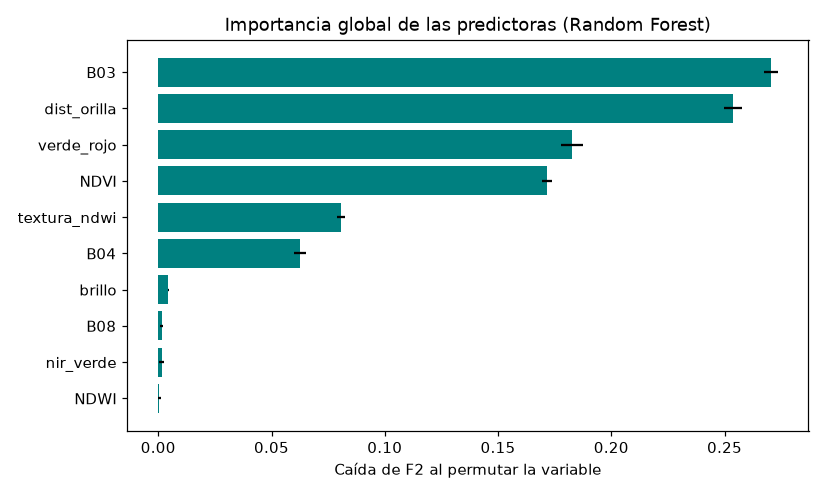
\includegraphics[width=0.72\linewidth]{figuras/importancia_global.png}
  \caption{Importancia global por permutación sobre el conjunto de prueba.}
\end{figure}

\begin{figure}[H]
  \centering
  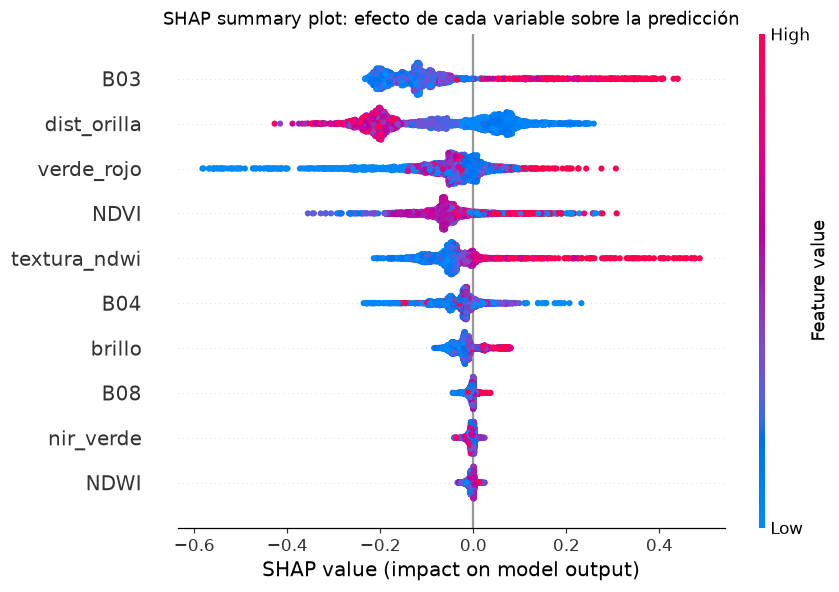
\includegraphics[width=0.8\linewidth]{figuras/shap_summary.png}
  \caption{SHAP summary plot. Cada punto es un píxel; el color indica si el valor de la variable es alto o bajo y
  la posición horizontal cuánto empujó esa variable la predicción.}
\end{figure}

Los dos métodos coinciden en el orden. Mandan la reflectancia en el verde y la distancia a la orilla, seguidas del
cociente verde-rojo, el NDVI y la textura del NDWI. En el extremo opuesto, el NDWI, el cociente infrarrojo-verde y
B08 no aportan prácticamente nada, con caídas de F2 por debajo de 0.002. Que el NDWI resulte inútil tiene sentido:
todas las observaciones ya son agua, así que dentro del lago esa variable casi no varía.

\begin{itemize}
  \item \textbf{B03 alto empuja hacia alta presencia} (correlación 0.82). Es el resultado más físico de todos: la
  cianobacteria dispersa luz en el verde, así que el agua florecida se ve más verde y más brillante. El brillo
  general apunta en el mismo sentido, con 0.79.
  \item \textbf{La textura del NDWI alta también empuja hacia arriba} (0.85), lo que confirma la intuición con que
  se construyó esa variable: la floración es manchada y deja vecindarios heterogéneos, mientras que el agua limpia
  es uniforme.
  \item \textbf{La distancia a la orilla funciona al revés} (correlación $-0.83$): mientras más cerca de la ribera
  está el píxel, más sube la predicción. Coincide con lo encontrado en la Parte I, donde la floración se acumula en
  la ribera norte de Amatitlán y en la desembocadura del río Villalobos.
  \item \textbf{El cociente verde-rojo y el NDVI empujan hacia arriba de forma más débil} (0.33 y 0.09) y su efecto
  no es monótono: contribuyen en combinación con las demás variables, no por sí solas.
\end{itemize}

Ambientalmente, el modelo reconoce una floración como agua más verde, más brillante, de textura irregular y cercana
a la orilla, que es una descripción razonable de una mancha de cianobacteria vista desde arriba. Hay, sin embargo,
una advertencia en ese resultado: que la distancia a la orilla sea la segunda variable más influyente significa que
buena parte de la decisión no es espectral sino geográfica. El modelo aprendió dónde suele haber floración, no solo
cómo se ve, y eso explica por qué no logra transferirse al otro lago, donde la geometría de la ribera y la
ubicación de las zonas afectadas son distintas.

\section{Mapas predictivos}

Para llevar las predicciones al mapa se recalculan las predictoras de todos los píxeles válidos de una imagen, no
solo de la muestra utilizada para modelar, y se coloca la probabilidad estimada de vuelta en la malla del raster.
Como el modelo se entrenó con el 70\% de una muestra del 4\%, apenas un 2.8\% de los píxeles mostrados participó
en el entrenamiento, de modo que el mapa es prácticamente fuera de muestra. La escala distingue cuatro niveles:
probabilidad muy baja por debajo de 0.25, baja entre 0.25 y 0.5, alta entre 0.5 y 0.75 y muy alta por encima
de 0.75.

\begin{figure}[H]
  \centering
  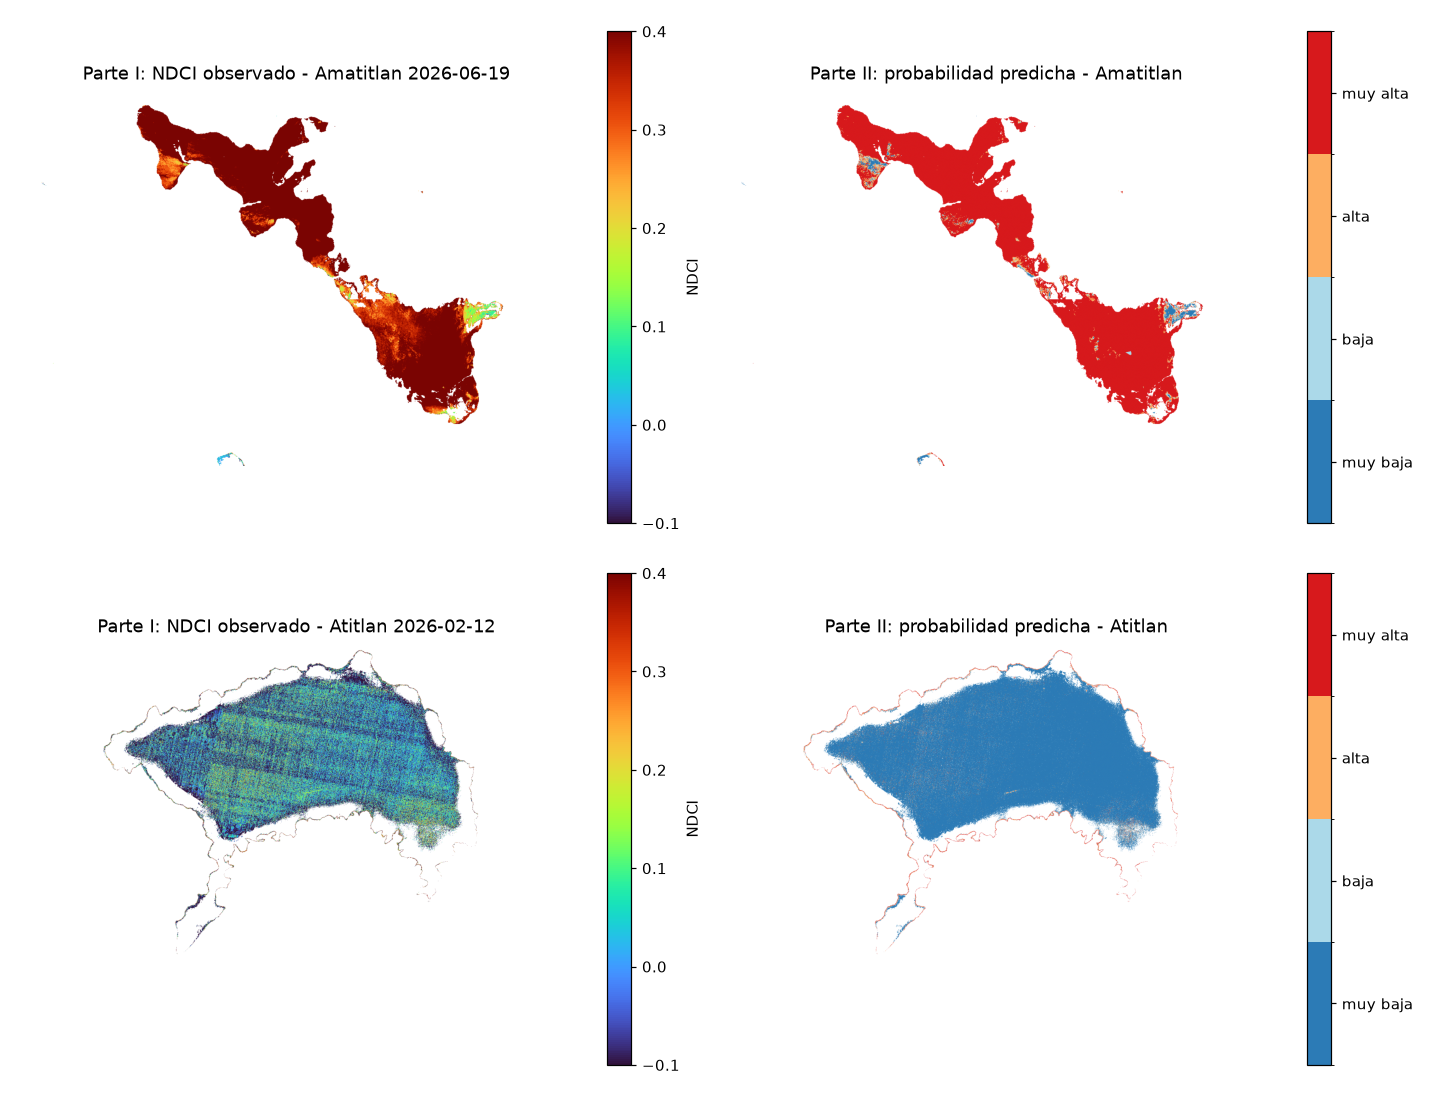
\includegraphics[width=0.92\linewidth]{figuras/comparacion_ndci_prediccion.png}
  \caption{Índice de cianobacteria observado en la Parte I frente a la probabilidad predicha por el modelo, para
  la misma fecha en cada lago.}
\end{figure}

\begin{table}[H]
  \centering
  \small
  \begin{tabular}{llrrrrrr}
    \toprule
    Lago & Fecha & Aciertos $-$ & Aciertos $+$ & Falsos $+$ & Falsos $-$ & Recall & Precisión \\
    \midrule
    Amatitlán & 2026-06-19 & 3,629   & 126,115 & 2,909  & 2,104 & 0.984 & 0.977 \\
    Atitlán   & 2026-02-12 & 853,795 & 11,242  & 14,953 & 9,654 & 0.538 & 0.429 \\
    \bottomrule
  \end{tabular}
  \caption{Aciertos y errores sobre la imagen completa de cada lago.}
\end{table}

En Amatitlán, el 19 de junio de 2026, el modelo reproduce casi exactamente la floración observada: sobre 134,757
píxeles detecta el 98.4\% de los positivos reales con una precisión del 97.7\%, y el mapa de errores muestra el
lago verde de lado a lado. Frente al mapa de NDCI de la Parte I la coincidencia es directa, lo que confirma que la
reconstrucción espacial es correcta.

En Atitlán, el 12 de febrero de 2026, el panorama cambia. Con solo 2.3\% de positivos reales, el modelo recupera el
53.8\% de ellos y acierta en el 42.9\% de sus alarmas. Es el escenario realista: cuando la clase positiva es rara y
espectralmente marginal, el mismo modelo que funciona en un lago florecido se vuelve poco confiable.

\begin{figure}[H]
  \centering
  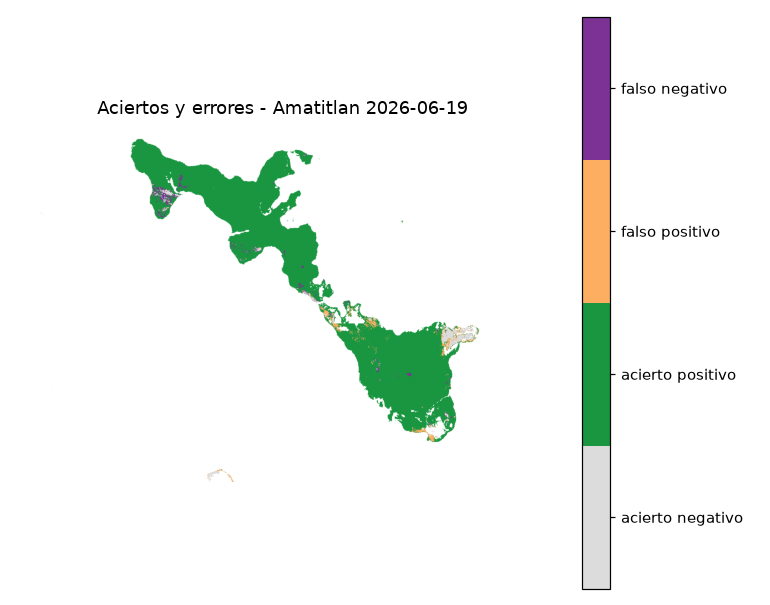
\includegraphics[width=0.49\linewidth]{figuras/mapa_errores_Amatitlan.png}
  \hfill
  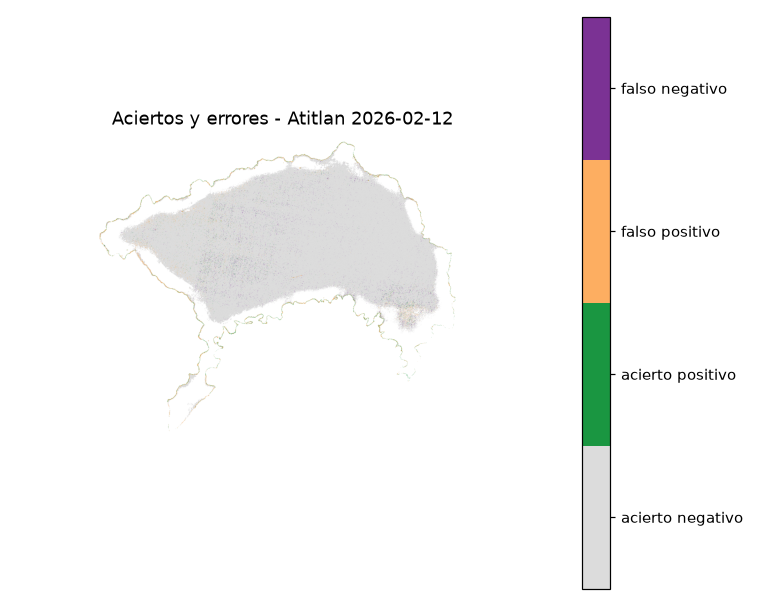
\includegraphics[width=0.49\linewidth]{figuras/mapa_errores_Atitlan.png}
  \caption{Distribución espacial de aciertos y errores en ambos lagos.}
\end{figure}

\subsection{Patrones espaciales del error}

El error no se reparte al azar dentro del lago: se concentra en la orilla.

\begin{table}[H]
  \centering
  \small
  \begin{tabular}{lrrrr}
    \toprule
    & \multicolumn{2}{c}{Amatitlán} & \multicolumn{2}{c}{Atitlán} \\
    \cmidrule(lr){2-3} \cmidrule(lr){4-5}
    Distancia a la orilla & Error total & Falsos $+$ & Error total & Falsos $+$ \\
    \midrule
    0 a 100 m      & 6.71\% & 5.01\% & 14.88\% & 13.29\% \\
    100 a 250 m    & 3.76\% & 1.57\% & 2.07\%  & 1.01\%  \\
    250 a 500 m    & 1.53\% & 0.48\% & 2.28\%  & 1.39\%  \\
    500 a 1000 m   & 0.43\% & 0.17\% & 1.78\%  & 0.80\%  \\
    Más de 1000 m  & ---    & ---    & 1.45\%  & 0.35\%  \\
    \bottomrule
  \end{tabular}
  \caption{Tasa de error según la distancia a la ribera. En Amatitlán la última franja tiene apenas 68 píxeles y
  se omite por no ser interpretable.}
\end{table}

En Atitlán los primeros cien metros desde la ribera concentran un 14.88\% de error, de los cuales 13.29 puntos son
falsos positivos, mientras que más allá de un kilómetro el error baja a 1.45\%. En Amatitlán ocurre lo mismo en
menor escala, 6.71\% contra 0.43\%. La causa es la mezcla dentro del píxel: un cuadro de 10 metros pegado a la
ribera combina agua con vegetación, y esa mezcla se parece espectralmente a una floración. Es el mismo artefacto
identificado en la Parte I, ahora cuantificado.

Por zonas del lago el reparto también es desigual y resulta revelador. En Amatitlán la mitad sur, que es la cuenca
más limpia, concentra los falsos positivos con 4.30\%, mientras que la mitad norte, la más cargada, concentra los
falsos negativos con 2.37\%: el modelo suaviza el gradiente norte-sur, exagera en la mitad limpia y se queda corto
en la más afectada. En Atitlán la mitad sur tiene 6.66\% de error frente a 2.07\% en la norte, porque es donde
están las bahías y la costa más recortada, de modo que hay proporcionalmente más píxeles de borde.

Para el uso práctico esto se traduce en una recomendación concreta: las alertas deberían ignorar la franja de los
primeros cien metros de ribera, o al menos tratarla por separado, porque ahí se produce la mayoría de las falsas
alarmas.

\section{Análisis y conclusiones}

\subsection{¿Sirve el modelo como herramienta de apoyo?}

Sirve como apoyo dentro de un lago que ya se está monitoreando, no como sustituto del muestreo ni como detector que
se pueda trasladar de un lago a otro. La evidencia sostiene las tres partes de esa afirmación.

A favor: con partición aleatoria el Random Forest alcanza F2 de 0.793 y ROC-AUC de 0.982, y al pasar a validación
espacial por bloques de un kilómetro solo baja a F2 de 0.744 con ROC-AUC de 0.973. Esa caída moderada indica que el
modelo aprendió algo más que la vecindad inmediata de sus píxeles de entrenamiento. En el mapa de Amatitlán del 19
de junio recupera el 98.4\% de la superficie afectada, que es justo lo que se le pediría a una herramienta de
alerta temprana.

En contra: la validación temporal, que es la que imita el uso real de predecir una fecha nueva, deja al Random
Forest en F2 de 0.586, muy por debajo de lo que sugería la partición aleatoria. Y la generalización entre lagos
fracasa por completo, con un F2 máximo de 0.090 al entrenar en Atitlán y evaluar en Amatitlán, y de 0.073 en la
dirección contraria. En Atitlán, en una fecha tranquila, el modelo detecta apenas la mitad de los positivos y menos
de la mitad de sus alarmas son correctas.

La conclusión operativa es que el modelo sirve para priorizar dónde tomar muestras y para vigilar de forma continua
un lago que ya tiene etiquetas propias, pero no para declarar limpio un cuerpo de agua ni para aplicarse tal cual en
un lago donde no fue entrenado. Cada lago necesita su propia calibración.

\subsection{Limitaciones encontradas}

\begin{itemize}
  \item \textbf{Las etiquetas no son mediciones de campo.} La variable respuesta se derivó del NDCI a través de la
  clorofila-a estimada, así que el modelo aprende a reproducir un índice satelital y no una concentración medida en
  laboratorio. Cualquier sesgo del índice se hereda.
  \item \textbf{La resolución espacial limita la ribera.} B05 es nativamente de 20 metros y se remuestreó a 10, y
  los píxeles de orilla mezclan agua con vegetación: ahí se concentra el error, hasta 14.88\% en los primeros cien
  metros de Atitlán.
  \item \textbf{Hay pocas fechas.} Son 11 por lago, 21 utilizables, y en Amatitlán solo una cae en época lluviosa.
  La validación temporal descansa en una única fecha retenida por lago, por lo que su métrica es la menos estable.
  \item \textbf{La nubosidad y la bruma cuestan datos.} El filtro sobre el infrarrojo cercano y la regla de
  cobertura mínima dejaron fuera una escena completa, la de Atitlán del 18 de enero de 2025, y recortan porciones
  de otras.
  \item \textbf{Los dos lagos no son comparables.} La prevalencia es de 39.9\% en Amatitlán y 1.1\% en Atitlán, y
  sus rangos de reflectancia tampoco coinciden, lo que explica que ningún modelo transfiera.
  \item \textbf{La metodología de validación importa más de lo que parece.} La partición aleatoria infla los
  resultados porque píxeles vecinos de la misma imagen son casi idénticos; los bloques de un kilómetro reducen ese
  efecto pero no lo eliminan, ya que la dependencia espacial se extiende más allá del bloque.
\end{itemize}

\subsection{Qué datos mejorarían el modelo}

\begin{itemize}
  \item \textbf{Muestreos físicos de clorofila-a y de toxinas.} Son la pieza que falta: permitirían entrenar contra
  concentraciones reales en lugar de contra un índice, y calibrar el umbral con mediciones locales en vez de tomarlo
  de una guía general.
  \item \textbf{Variables meteorológicas.} El viento explica hacia qué ribera se acumula la mancha, y la
  temperatura del aire y la lluvia de los días previos condicionan el crecimiento. Ninguna está hoy en el modelo.
  \item \textbf{Datos hidrológicos del río Villalobos}, en particular caudal y carga de nutrientes, que son el
  origen del problema en Amatitlán y hoy solo entran de forma indirecta mediante la distancia a la orilla.
  \item \textbf{Temperatura superficial del agua}, obtenible de la banda térmica de Landsat 8 y 9, que es uno de los
  factores que más influye en la proliferación.
  \item \textbf{Más fechas y más bandas.} Usar todas las pasadas disponibles de Sentinel-2 daría una serie temporal
  real, y las bandas SWIR B11 y B12 permitirían enmascarar nubes y bruma mucho mejor que el filtro actual. Para
  agua, el sensor OLCI de Sentinel-3 ofrece más bandas en el borde rojo, diseñadas para estimar clorofila.
\end{itemize}

\end{document}
